\documentclass[12pt, titlepage]{article}
\usepackage[margin=1in]{geometry}
\usepackage{amsmath}
\usepackage{pgfplots}
\pgfplotsset{compat=1.16}
\usepackage{parskip}
\usepackage{caption}
\usepackage{physics}
\usepackage{graphicx}
\usepackage{float}
\usepackage{url}

\date{Session: May 2020 \\ Subject: Mathematics \\ Word Count: 3328}
\title{The Application of a Taylor Series Approximation for \(\pi\) in a Related Rates Problem using a Solid of Revolution \bigskip \\  How well can Taylor series approximations for pi be applied in rates of change of cyclical objects?}

\begin{document}
\maketitle
\tableofcontents
\newpage

\section{Introduction}
Irrational numbers like \(\pi\) have been approximated ever since they've been first discovered. Nowadays, mathemticians have become so dependent on technology, that they have taken for granted the ease of which they can approximate irrational numbers. Modern calculators have made it a lot easier to approximate irrational numbers like e and \(\pi\). However, when mathemticians rely on technology to do their calculations, they are limited to the accuracy of said technology. For example, a Ti-83 calculator can only approximate \(\pi\) to 9 decimal places, ``3.141592654". If a better approximation is necessary, a more accurate calculator would be required to solve the problem. Often overlooked approximation methods can be just as accurate as a calculator, and have the potential benefit of being modified to manipulate accuracy as necessary.

As a young child, I was always interested in irrational numbers like pi and the square root of two. In my IB mathematics class, I learned that although irrational numbers have never ending decimals that don't even repeat, that they can be approximated using series. I was simply confounded by the idea that adding an endless amount of numbers could result in a finite number, much less an irrational number. My first meanvingful interaction with a toilet was when I pondered about the curvature of a toilet. I hypothesized that there was no way the volume of the toilet could be a whole number, yet humans are able to make them nonetheless. This led me to the investigation of approximating curves using Taylor series and to the research question: How well can Taylor series approximations for pi be applied in rates of change of cyclical objects?

\subsection{What is a Taylor Series?}
A Taylor series is an approximation method that can be used to approximate functions and irrational numbers. According to Ron Larson, if a function f has derivatives of all orders at x = c, then the Taylor series for f at c is: (Larson 613)
\begin{equation}
  \sum_{n=0}^{\infty} \frac{f^{(n)}(c)}{n!} \, (x-c)^{n} = f(c) + f'(c)(x-c) + ... +  \frac{f^{(n)}(c)}{n!}
\end{equation}

It is possible to apply this formula where f(n) is the nth derivative to derive the Taylor series for arctan(x) which to approximate \(\pi\)

To demonstrate the utility of approximating with Talor series, the paper will explore the calculations of the volume and rate of water flowing into a toilet bowl. Firstly, rotating a parabola into a solid of revolution will be used to model the structure of the bowl. In this way, manipulation of the upper bound of integration will allow the volume of this bowl to somewhat resemble that of a curved toilet bowl. It is important to note that a normal toilet bowl's structure is not perfectly parabolic. However, this model will defy standard conventions for simplicity. I predict that using a Taylor series will prove to be very accurate and easy to calculate by hand for approximating pi. 

\subsection{Power of Taylor Series}
Taylor series can turn transcendental numbers into polynomials. This is revolutionary in that numbers like \(e\) and \(\pi\) can be viewed not only as irrational numbers, but as algebraic functions.

To illustrate the graphical property of a Taylor series, the transcendental function \(e^{x}\) will be approximated.
\begin{figure}[H]
\centering
    \caption[]{\(y=e^x\)}
\begin{tikzpicture}
\begin{axis}
    [xmin=-5,
    ]
    \addplot[color=orange]{e^x};
    \node [color=blue, smooth, ultra thick, font=\Large] at (4,150) {$y=e^x$};
\end{axis}
\end{tikzpicture}
\end{figure}

The Taylor series representation of \(e^{x}\) is  
\begin{equation}
  \sum_{n=0}^{\infty} \frac{x^{n}}{n!}
\end{equation}

The series was derived from the general formula of a Taylor series.
\begin{equation}
  \sum_{n=0}^{\infty} \frac{f^{(n)}(c)}{n!} \, (x-c)^{n} = f(c) + f'(c)(x-c) + ... +  \frac{f^{(n)}(c)}{n!}
\end{equation}

Centering the Taylor series at the point c = 0 results in a Macluarin series. Since the derivative of \(e^{x}\) is \(e^{x}\), \(f^{(n)}(0)\) is always equal to 1.

The series simplifies to:
\begin{equation}
  \sum_{n=0}^{\infty} \frac{x^{n}}{n!}
\end{equation}

\pagebreak
Using a first order or linear approximation of P(1) = 1 + x:
\begin{figure}[H]
\centering
    \caption[]{\(y=e^x\) and first order approximation}
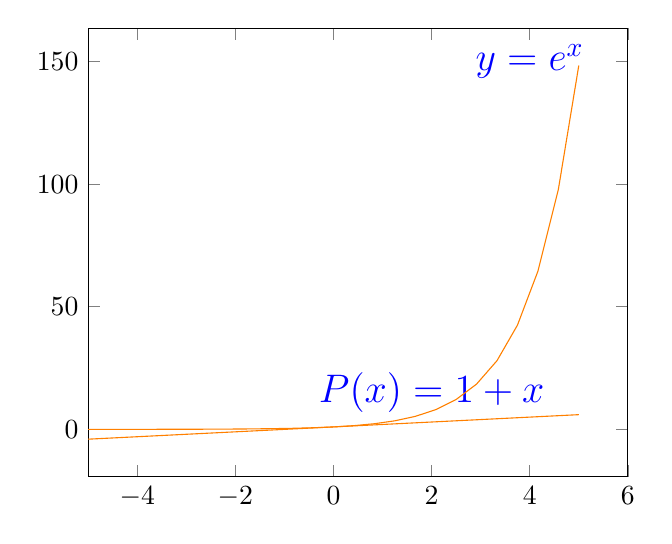
\begin{tikzpicture}
\begin{axis}
    [xmin=-5,
    ]
    \node [color=blue, smooth, ultra thick, font=\Large] at (2,15) {$P(x)=1+x$};
    \node [color=blue, smooth, ultra thick, font=\Large] at (4,150) {$y=e^x$};
    \addplot[color=orange]{e^x};
    \addplot[color=orange]{1+x};
\end{axis}
\end{tikzpicture}
\end{figure}

Not only can Taylor polynomials be used to approximate irrational numbers graphically, they can also be approximated at a point x to approximate the value f(x) of an irrational number. This can be done by plugging the x value into the Taylor polynomial. Plugging in x = 1 into the function of \(e^x\) will  approximate \(e^1\) or e. 

First, the first order approximation is P(x) = 1 + x. Plugging in 1 into the Taylor polynomial T(1) = 1 + 1 = 2. Let's note that the Ti-83 approximates e as 2.718281828

Using a second order approximation:
\begin{equation}
  P(2) = \sum_{n=0}^{2} \dfrac{x^{n}}{n!} = 1 + x + \dfrac{x^{2}}{2!}:
\end{equation}

\begin{figure}[H]
\centering
    \caption[]{\(y=e^x\) and second order approximation}
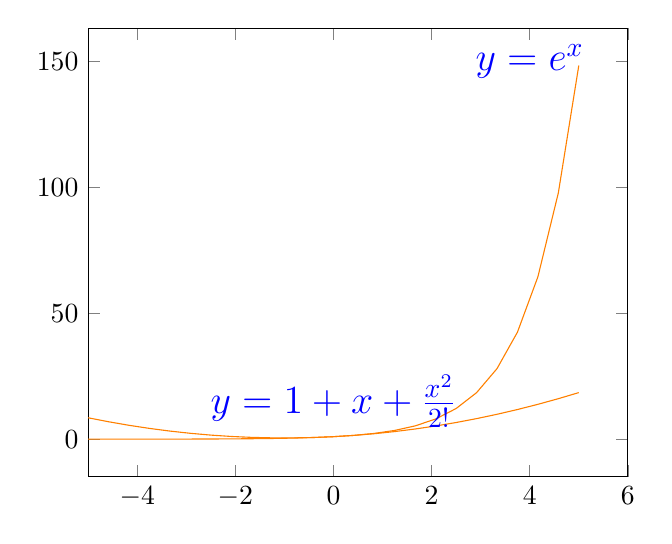
\begin{tikzpicture}
\begin{axis}
    [xmin=-5,
    ]
\addplot[color=orange]{e^x};
\addplot[color=orange]{1+x+(x^2)/2};
    \node [color=blue, smooth, ultra thick, font=\Large] at (0,15) {$y=1+x + \frac{x^2}{2!}$};
    \node [color=blue, smooth, ultra thick, font=\Large] at (4,150) {$y=e^x$};
\end{axis}
\end{tikzpicture}
\end{figure}

Higher order approximations are more accurate than lower order approximations, in this case the second approximation is more accurate than the first and thus matches the curve of the function f(x) = \(e^{x}\) more accurately. The second order approximation for \(e^{x}\) is T(x) = 1 + x + \(\dfrac{x^2}{2!}\). Plugging in 1 into the Taylor polynomial T(1) = 1 + 1 + 0.5 = 2.5. As shown by the graph and numerical value of error, the function approximation is getting closer and closer to the value of e as more terms are added.

Using a third order approximation of P(3) = 1 + x + \(\dfrac{x^{2}}{2!}\) + \(\dfrac{x^{3}}{3!}\):
\begin{figure}[H]
\centering
    \caption[]{\(y=e^x\) and third order approximation}
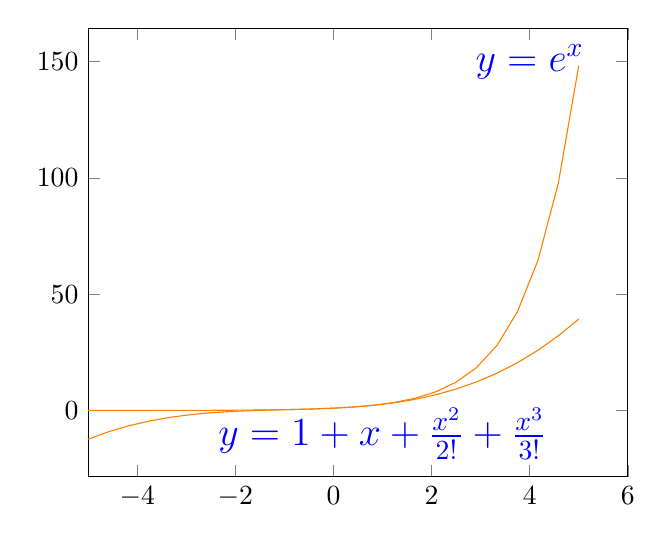
\begin{tikzpicture}
\begin{axis}
    [xmin=-5,
    ]
    \node [color=blue, smooth, ultra thick, font=\Large] at (1,-10) {$y=1+x + \frac{x^2}{2!} + \frac{x^3}{3!}$};
    \node [color=blue, smooth, ultra thick, font=\Large] at (4,150) {$y=e^x$};
    \addplot[color=orange]{e^x};
    \addplot[color=orange]{1+x+(x^2)/2+(x^3)/6};
\end{axis}
\end{tikzpicture}
\end{figure}

An 8 term approximation is strikingly similar to the graph of \(y = e^{x}\)
\begin{figure}[H]
\centering
    \caption[]{\(y=e^x\) and eigth order approximation}
\begin{tikzpicture}
\begin{axis}
    [xmin=-5,
    ]
\addplot[color=orange]{e^x};
\addplot[color=orange]{1+x+(x^2)/2+(x^3)/6+(x^4)/24+(x^5)/120+(x^6)/720+(x^7)/5040+(x^8)/40320};
\node [color=blue, smooth, ultra thick, font=\Large] at (4,150) {$y=e^x$};
\end{axis}
\end{tikzpicture}
\end{figure}

An eighth order approximation for is T(x) = 1 + x + \(\dfrac{x^2}{2!}\) + \(\dfrac{x^3}{3!}\)
+ \(\dfrac{x^4}{4!}\) + \(\dfrac{x^5}{5!}\) + \(\dfrac{x^6}{6!}\) + \(\dfrac{x^7}{7!}\) + \(\dfrac{x^8}{8!}\)

Plugging in 1 into the 8th degree Taylor polynomial:
\begin{equation}
  1 + 1 + \dfrac{1^2}{2!} + \dfrac{1^3}{3!} + \dfrac{1^4}{4!} + \dfrac{1^5}{5!} + \dfrac{1^6}{6!} + \dfrac{1^7}{7!} + \dfrac{1^8}{8!} \approx 2.71827877
\end{equation}

This value is even closer to the value of e. In fact, the two functions are almost indistinguishable on the domain [0,5]. As more and more terms are included in the approximation, the more closer and the more accurate the approximation gets to what it's trying to approximate. In this way, Taylor series could prove to be a useful way to approximate \(\pi\). In fact, I predict that the Taylor series derived  will be able to beat the approximation of the Ti-83 calculator in accuracy.

\section{Finding a Taylor Series for \(\pi\)}
Since \(tan(\frac{\pi}{4})\) = 1, then \(arctan(1)= \frac{\pi}{4}\). It is now possible to plug in the value of x = 1 into the arctan equation, with the intention that arctan(1) = pi/4. It is then possible to multiply this approximation by 4 to get an approximation for pi.

\begin{figure}[H]
\centering
    \caption[]{f(x) = arctan(x)}
\begin{tikzpicture}
\begin{axis}
    [    domain = -10:10,
    xmin=-10,
    xmax =10,
    ymin = -5,
    ymax = 5,
    xscale = 1, yscale = 1,
    axis lines = center,
    ]
    \addplot[color=orange]{rad(atan(x))};
\end{axis}
\end{tikzpicture}
\end{figure}

\begin{equation}
  f(x) = arctan(x)
\end{equation}

The first derivative of arctan(x) is 
\begin{equation}
f'(x) = \frac{1}{1 + x^{2}}
\end{equation}

\pagebreak
The derivative of arctan(x) can be derived with this triangle using basic trigonometry and calculus:
\begin{figure}[H]
\centering
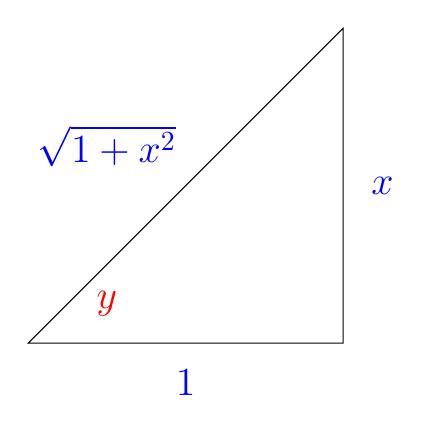
\begin{tikzpicture}
\draw (0,0)
  -- (4,0) 
  -- (4,4) 
  -- cycle;
  \node [color=blue, smooth, ultra thick, font=\Large] at (4.5,2) {$x$};
  \node [color=blue, smooth, ultra thick, font=\Large] at (2,-.5) {$1$};
  \node [color=blue, smooth, ultra thick, font=\Large] at (1,2.5) {$\sqrt{1 + x^2}$};
    \node [color=red, smooth, ultra thick, font=\Large] at (1,.5) {$y$};
\end{tikzpicture}
\end{figure}

This triangle allows the derivation of:
\begin{equation}
 tan(y) = x
\end{equation}

Solving for y results in arctan
\begin{equation}
  y = arctan(x)
\end{equation}

To Calculate the derivative of tan(y), we use a trig identity to define it in terms of sin(y) and cos(y).
\begin{equation}
 tan(y) = \frac{sin(y)}{cos(y)}
\end{equation}

Applying the diferential operator on both sides.
\begin{equation}
  \frac{d}{dx} tany = \frac{d}{dx} \frac{sin(y)}{cos(y)}
\end{equation}

Taking the derivative of both sides
\begin{equation}
  \frac{d}{dx} tany = \frac{d}{dx} \frac{sin(y)}{cos(y)}
\end{equation}

Applying the quotient rule:
\begin{equation}
  \frac{d}{dx} tany = \frac{cos(y)cos(y) - sin(y)(-sin(y))}{cos(y)cos(y)}
\end{equation}

Simplifying by combining like terms
\begin{equation}
  \frac{d}{dx} tany = \frac{cos^{2}(y) + sin^{2}(y)}{cos^{2}(y)}
\end{equation}

Although it is possible to use Pythagorean's identity to further simplify \(cos^{2}(y) + sin^{2}(y) = 1\) to get \(\dfrac{1}{cos^{2}(y)} = sec^{2}(y)\), simplifying by splitting into two fractions will be used instead. 
\begin{equation}
  \frac{d}{dx} tany = 1 + tan^{2}(y)
\end{equation}

At first, this does not seem useful as the derivative of tan(y) is defined in terms of tan(y), however remember that we defined y = arctan(x).

Now that the derivative of tan(y) was derived, it is possible to diferentiate implicitly on both sides.
\begin{equation}
 \frac{d}{dx} tan(y) = \frac{d}{dx} x
\end{equation}

Chain Rule results in a dy/dx
\begin{equation}
 1 + tan^{2}(y) \frac{dy}{dx}  = 1
\end{equation}

Solving for dy/dx
\begin{equation}
 \frac{dy}{dx}  = \frac{1}{1 + tan^{2}(y)}
\end{equation}

Substituting tan(y) for x to find the derivative of y = arctan(x).
\begin{equation}
 \frac{dy}{dx}  = \frac{1}{1 + x^{2}}
\end{equation}

Calculating the second derivative using Power Rule.
\begin{equation}
    f"(x) = \frac{-2x}{(1+x^{2})^{2}}
\end{equation}

The 3rd derivative of arctan(x) is:
\begin{equation}
    f^{(3)}(x) = \frac{2(3x^{2}-1)}{(x^{2}+1)^{3}}
\end{equation}

Even though plugging in x = 0 to even termed derivatives results in 0, the derivatives become more and more complex with higher and higher derivatives. Using Taylor's formula to make a Taylor series for arctan(x) becomes less efficient as the order of approximation increases and thus another method to derive a Taylor series for arctan(x) will be needed.

\subsection{Deriving a Taylor Series for arctan(x)}
Starting with arctan(x),
\begin{equation}
  f(x) = arctan(x)
\end{equation}

Taking the derivative of arctan(x),
\begin{equation}
f'(x) = \frac{1}{1 + x^{2}}
\end{equation}

The derivative of arctan(x) has the form of the function:
\begin{equation}
    g(u) = \frac{1}{1+u}
\end{equation}
Where u = \(x^2\)

This function is represented by the series:
\begin{equation}
    g(x) = \sum_{n=0}^{\infty} (-1)^{n}x^{n}
\end{equation}

Substituting \(x^{2}\) for u. 
\begin{equation}
    g(x^{2}) = \sum_{n=0}^{\infty} (-1)^{n}x^{2n}
\end{equation}

Therefore f'(x) can be represented by the series:
\begin{equation}
f'(x) = \frac{1}{1 + x^{2}} = \sum_{n=0}^{\infty} (-1)^{n}x^{2n}
\end{equation}

To derive the series for f(x) = arctan(x), integrate the series for f'(x)
\begin{equation}
    arctan(x) = \int \frac{1}{1+x^{2}} \; dx + C = \sum_{n=0}^{\infty} (-1)^{n}\frac{x^{2n+1}}{2n+1} + C
\end{equation}

At x = 0, arctan(0) = 0, which allows solving for c which equals C = 0,
\begin{equation}
    arctan(x) = \sum_{n=0}^{\infty} (-1)^{n}\frac{x^{2n+1}}{2n+1} 
\end{equation}

\subsection{Constructing a series representation for \(\pi\)}
The Taylor series constructed previously for arctan(x) is:
\begin{equation}
    arctan\,x = \sum^{\infty}_{n=0} \frac{(-1)^{n}\,x^{2n+1}}{2n+1}
\end{equation}

It is convenient that the function arctan\,x evaluated at 1 is \(\dfrac{\pi}{4}\).
\begin{equation}
    arctan(1) = \frac{\pi}{4}
\end{equation}

Substituting x for 1.
\begin{equation}
    arctan(1) = \frac{\pi}{4} = \sum_{n=0}^\infty{ \frac{(-1)^n}{2n+1}}
\end{equation}

Writing out the first 4 terms of this series, it is easy to tell that this is an alternating series; the \((-1)^{n}\) causes the terms to alternate from positive to negative.
\begin{equation}
    \frac{\pi}{4} =\sum_{n=0}^\infty{ \frac{(-1)^n}{2n+1} = 1 - \frac{1}{3} + \frac{2}{5} - \frac{1}{7} + ... }
\end{equation}

Solving for pi.
\begin{equation}
    \pi = 4 \sum_{n=0}^\infty{ \frac{(-1)^n}{2n+1} = 4 - \frac{4}{3} + \frac{8}{5} - \frac{4}{7} + ... }
\end{equation}

According to Hlawitschka, Taylor series may not be accurate or even be erroneous if the series diverges (Hlawitschka). Christine Palmer claims that ``In practice the Taylor series does converge to the function for most functions of interest, so that the Taylor series for a function is an excellent way to work that function" (Palmer). Even so, as per Hlawitschka, it is necessary to prove that the Taylor series representation of arctan(x) is convergent by using the Alternating Series Test.

\section{Alternating Series Test}
The alternating series test will be used to see if the series for arctan(x) is convergent. According to Ron Larson, an alternating series converges when the two conditions listed below are met (Larson 567).

First, the limit of the nth term must equal zero.
\begin{equation}
    \lim_{n \to \infty} a_{n} = 0
\end{equation}

And the function must be decreasing.
\begin{equation}
    a_{n+1} \leq a_{n}, \textrm{for all} \; n
\end{equation}

\subsection{Nth Term Test}
Calculating the limit of the nth term will test whether the series meets the first requirement.
\begin{equation}
    \lim_{n \to \infty} \frac{1}{2n+1} = 0     
\end{equation}

The limit of the nth term as n approaches infinity is zero as the denominator grows increasingly large while the numerator remains constant.

\subsection{Terms are non-increasing}
\(a_{n+1} \leq a_{n}\), therefore the function is decreasing for all n. 
\begin{equation}
    a_{n+1} = \frac{1}{2(n+1) + 1} = \frac{1}{2n+3} \leq \frac{1}{2n+1} = a_{n}
\end{equation}

Therefore the series converges by the Alternating Series Test.

\section{Absolute Convergence}
The definition of absolute convergence will determine whether the series derived for the function arctan(x) is absolutely convergent.

According to Ron Larson, absolute convergence is defined as: 

``The series \(\sum a_{n}\) is absolutely convergent when \(\sum \abs{a_{n}}\) converges" (Larson 570).

\subsection{Testing for absolute convergence}
The series derived for arctan(x).
\begin{equation}
    \sum_{n=0}^{\infty} (-1)^{n} \frac{x^{2n+1}}{2n+1}
\end{equation}

Taking the absolute value of the series.
\begin{equation}
    \sum_{n=0}^{\infty}   \left |  (-1)^{n} \frac{x^{2n+1}}{2n+1} \right |
\end{equation}

In other words, it is necessary to test if the non alternating part is convergent.
\begin{equation}
    \sum_{n=0}^{\infty}   \left |\frac{1}{2n+1} \right |
\end{equation}

This behaves like the harmonic series \(\sum\limits_{n=0}^{\infty} \dfrac{1}{n}\) which is divergent. Therefore the alternating series for arctan(x) is not absolutely convergent. This means that it is necessary to check the interval convergence to determine if the series can be used to approximate pi at x = 1 by checking if x = 1 falls into the interval in which the series representation of arctan(x) converges.

\subsection{Using the Ratio Test}
The ratio test will be used to determine the interval of convergence. The interval of convergence is ``the set of real numbers x for which a power series converges" (Strang 6). This helps determine if the series is convergent at x = 1.

The series derived for arctan(x).
\begin{equation}
    \sum_{n=0}^{\infty} (-1)^{n} \frac{x^{2n+1}}{2n+1}
\end{equation}
 
The Ratio Test is a limit test of the ratio between the n + 1 term and the nth term which allows testing for convergence. If \(L < 1\), then the series converges absolutely. If \(L > 1\), then the series is divergent and if L = 1, then the test is inconclusive.
\begin{equation}
    L = \lim_{n \to \infty} \left |\frac{a_{n+1}}{a_{n}} \right | < 1
\end{equation}

Plugging in the nth + 1 term and then multiplying by the reciprocal of the nth term.
\begin{equation}
    \lim_{n \to \infty} \left |\frac{(-1)^{n}x^{2(n+1)+1}}{2(n+1)+1} \cdot \frac{2n+1}{(-1)^{n}x^{2n+1}} \right | < 1
\end{equation}

As there are absolute value bars, it is possible to ignore the alternating parts because they will not affect the value of the function.
\begin{equation}
    \lim_{n \to \infty} \left |\frac{x^{2n+3}}{2n+3} \cdot \frac{2n+1}{x^{2n+1}} \right | < 1
\end{equation}

Simplifying and taking \(x^{2}\) out of the limit,
\begin{equation}
    x^{2} \lim_{n \to \infty} \left |\frac{2n+1}{2n+3} \right | < 1
\end{equation}

\begin{equation}
    x^{2} < 1
\end{equation}

As shown previously, the series is convergent within \(-1 < x < 1\), however it is still necessary to check the bounds for convergence. If the series proves to not converge at x=1, then the series is not a good predictor of \(\pi\) as the appproximation relies on the fact that arctan(1) = pi/4.

\subsection{Checking the bounds}
\begin{equation}
    \sum_{n=0}^{\infty} (-1)^{n} \frac{x^{2n+1}}{2n+1}
\end{equation}

Plugging in x = -1,
\begin{equation}
    \sum_{n=0}^{\infty} (-1)^{n} \frac{(-1)^{2n+1}}{2n+1}
\end{equation}

Combining the alternating parts results in:
\begin{equation}
    \sum_{n=0}^{\infty} (-1)^{3n+1} \frac{1}{2n+1}
\end{equation}

Plugging in x = 1:
\begin{equation}
    \sum_{n=0}^{\infty} (-1)^{n} \frac{(1)^{2n+1}}{2n+1}
\end{equation}

Simplifying,
\begin{equation}
    \sum_{n=0}^{\infty} (-1)^{n} \frac{1}{2n+1}
\end{equation}

These both pass the alternating series test as the limit of their nth term is zero and the series is always decreasing. Therefore the interval of convergence for arctan(x) is \( -1 \leq x \leq 1 \). This means that the Taylor series for arctan(x) can be approximated at x=1 to approximate \(\pi/4\).

\section{Finding Error of Approximations}
The more accurate an approximation needs to be, the more terms will be needed in the Taylor polynomial. However, this is a more difficult task than just plugging in values into the derived Taylor polynomial because the goal is to figure out just how accurate or long the Taylor polynomial needs to be to reach a certain level of accuracy.

According to Christine Palmer, ``f(x) = Tn(x) + Rn(x)" where Tn(x) is the approximation and Rn(x) is the error (Palmer). However, solving for Rn(x) directly would not be beneficial because f(x) is irrational.
According to Calculus for AP, ``If a convergent alternating series satisfies the condition \(a_{n+1} \leq a_{n} \), then the absolute value of the remainder \(R_{n}\) involved in approximating the sum S by \(S_{n}\) is less than (or equal to) the first neglected term" (Larson 569).

That is:
\begin{equation}
  \abs{S - S_{n}} = \abs{R_{n}} \leq a_{n + 1}
\end{equation}

This concept allows us to figure out how many terms are needed to beat the Ti-83 calculator's approximation.

\subsection{Alternating Series Remainder}
The Taylor approximation for pi is:
\begin{equation}
  \pi = 4\sum_{n=0}^{x}{ \frac{(-1)^n}{2n+1}}
\end{equation}

The approximation using only one term is:
\begin{equation}
  P(0) = 4 \cdot \frac{1}{1} = 4
\end{equation}

It is possible to find the error by taking the absolute value of  the subtraction of the actual value of \(\pi\) by our approximation, in this case P(0) = 4. However, this is problematic as \(\pi\) is an irrational number that is being approximated in the first place. Instead, the error of the approximation can be found by using the Alternating Series Remainder.

The Alternating Series Remainder is the value of the next unused term.

The error of the first approximation using the next unused term is:
\begin{equation}
  \abs{R(0)} \leq \abs{\frac{-4}{3}} \leq \frac{4}{3}
\end{equation}

To continue, a two term approximation of \(\pi\) is:

\begin{equation}
  P(1) = 4 \cdot (\frac{1}{1} - \frac{1}{3}) = \frac{8}{3} 
\end{equation}

And this approximation has an error of:
\begin{equation}
  R(1) \leq  \abs{4 \cdot {\frac{(-1)^n}{2(2)+1}}} = \frac{4}{5} = 0.8
\end{equation}

\begin{figure}[H]
\centering
    \caption[]{f(x) = arctan(x) and two term approximation}
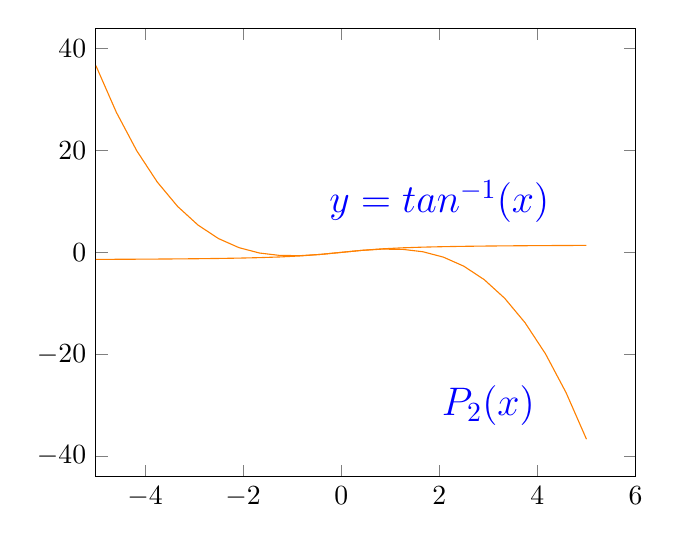
\begin{tikzpicture}
\begin{axis}
    [xmin=-5,
    ]
    \addplot[color=orange]{rad(atan(x))};
    \addplot[color=orange]{x - (x^3)/3}; 
    \node [color=blue, smooth, ultra thick, font=\Large] at (3,-30) {$P_{2}(x)$};
    \node [color=blue, smooth, ultra thick, font=\Large] at (2,10) {$y=tan^{-1}(x)$};
\end{axis}
\end{tikzpicture}
\end{figure}

A ninth order approximation or five term approximation has an error of 
\begin{figure}[H]
\centering
    \caption[]{f(x) = arctan(x) and ninth order approximation}
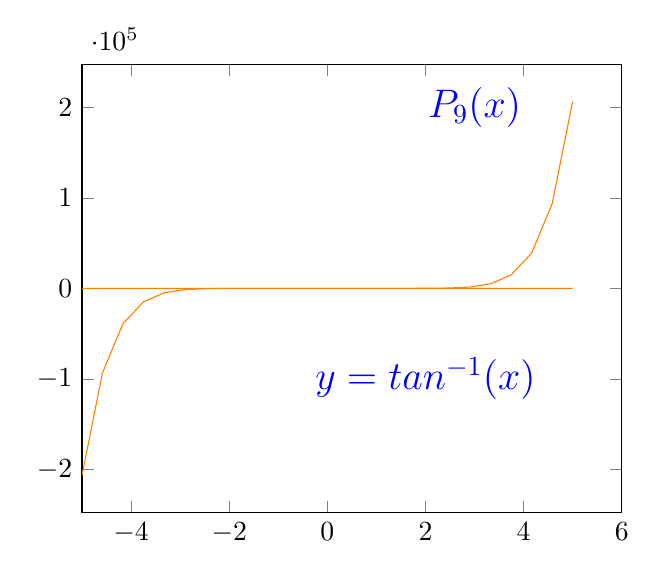
\begin{tikzpicture}
\begin{axis}
    [xmin=-5,
    ]
\addplot[color=orange]{rad(atan(x))};
\addplot[color=orange]{x - (x^3)/3 + (x^5)/5 - (x^7)/7 + (x^9)/9};
\node [color=blue, smooth, ultra thick, font=\Large] at (3,2 * 10^5) {$P_{9}(x)$};
    \node [color=blue, smooth, ultra thick, font=\Large] at (2,-10^5) {$y=tan^{-1}(x)$};
\end{axis}
\end{tikzpicture}
\end{figure}

As seen prior, the Taylor series gets more accurate the more terms it uses. It is important to note that the approximation can be either an over approximation or under approximation because the approximation is an alternating series. According to Lowry-Duda, ``the graph of the original function subtracted by the Taylor polynomial can be used as a graphical representation of error." (Lowry-Duda). This is another way to visually see the difference between the ninth order and two term approximation of arctan(x). 

\begin{figure}[H]
\centering
    \caption[]{error of two term approximation}
\begin{tikzpicture}
\begin{axis}
    [xmin=-5,
    ]
\addplot[color=orange]{rad(atan(x)) - x + (x^3)/3};
\end{axis}
\end{tikzpicture}
\end{figure}

\begin{figure}[H]
\centering
    \caption[]{error of ninth order approximation}
\begin{tikzpicture}
\begin{axis}
    [xmin=-5,
    ]
\addplot[color=orange]{rad(atan(x)) - x + (x^3)/3 - (x^5)/5 + (x^7)/7 - (x^9)/9};
\end{axis}
\end{tikzpicture}
\end{figure}

The graph of the error of the ninth order approximation is a lot closer to zero than the graph of the error of the two term approximation. This is further evidence that a Taylor series gets more accurate as more terms are added.

\subsection{Ti-83 and Wolfram Alpha's Approximation of \(\pi\)}
The Ti-83's approximation for \(\pi\) is: 3.141592654. This is accurate to 9 decimal places or \(10^{-9}\)

In order to calculate the least amount of terms that are needed to beat the Ti-83's approximation, I had to rely on a Python program to continually find the next unused term that would be less than or equal to \(10^{-9}\). See appendix for the Python program.

The output of the program is:
\begin{verbatim}
The approximation requires at least 1999999999 terms, 
and the next unused term is 
n = 2000000000
\end{verbatim}

The Wolfram Alpha approximation for \(\pi\) is:

3.141592653589793238462643383279502884197169399375105820974

This is accurate to 57 decimal places. A Taylor series approximation would need almost 2 billion terms to beat Wolfram Alpha's approximation of \(\pi\), rendering it impossibile to calculate using the Taylor series at this level of accuracy. In this way, although a Taylor series approximation of \(\pi\) can substitute technology for basic calculations, it is not as effective technology. The difficulty in using Taylor series is not only determing how many terms are needed but adding their partial sum. Without the aid of technology, a Taylor series would only be feasible if the approximation required no more than 20 terms. Since the Taylor series converges so slowly, more terms are required to reach a certain level of accuracy,

\subsection{More reasonable approximations}
A Taylor series with 2 terms has an error of less than or equal to 0.8.

Expanding the Taylor approximation to 12 terms reduces the error to less than or equal to 0.16. This is about as effective as approximating \(\pi\) as 3.

To get an approximation better than 3.14 or have an error less than or equal to 0.01, 199 terms are needed. 

\section{Related Rates Problem}
A toilet bowl is being filled with water at a constant rate of \(0.968 L/s\). At what rate is the level of water rising when the water in the tank is 2 cm deep?

\subsection{Modeling the toilet}
\begin{figure}[H]
\centering
  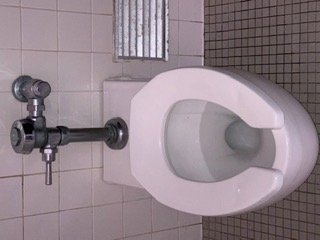
\includegraphics[angle=270]{toilet.jpeg}
    \caption{The toilet examined.}
\end{figure}

As noted earlier, flushing the toilet causes the rate of water flowing into the toilet to spike initially, then gradualy slowing down, until no more water flows into the toilet. However, for the sake of the related rates problem, a constant flush rate will be assumed as the priority is to apply our approximation to a real life problem. It is also important to note that the volume of the toilet is not completely filled with water.  

The graph of \(x^{2}\) will be used to model the curvature of the toilet and the cross section of the toilet bowl. More specifically, the solid of revolution around the y axis will create a toilet shaped bowl. 

\begin{figure}[H]
\centering
    \caption[]{\(y=x^2\)}
\begin{tikzpicture}
\begin{axis}
    [xmin=-5,
    ]
\addplot[color=orange]{x^2};
\end{axis}
\end{tikzpicture}
\end{figure}

Integrating area to get volume through the disc method.
\begin{equation}
    V = \int^y_0 \pi r^2\,dy
\end{equation}
Substituting the radius for \(\sqrt{y}\).
\begin{equation}
    V = \int^y_0 \pi \sqrt{y}^2\,dy  = \int^y_0 \pi y\,dy 
\end{equation}

Applying the first fundamental theorem of Calculus.
\begin{equation}
    V = \frac{ \pi y^2 }{2} \biggr \rvert^y_0 = \frac{\pi y^3}{2}
\end{equation}

\subsection{Finding the rate of change of volume}
In order to find the rate at which the volume of water flows from the toilet, the volume of a toilet as well as how long it takes the toilet to flush will need to be calculated. 

\pagebreak
The toilet in my school’s bathroom uses 13.2 L per flush. Using a stopwatch, I averaged how long it takes for twenty toilet flushes. 

\begin{center}
\begin{tabular}{rr}
Flush & Time (s \(\pm\) 0.01s)\\
\hline
1 & 14.25\\
2 & 15.00\\
3 & 14.60\\
4 & 14.05\\
5 & 14.75\\
6 & 15.91\\
7 & 16.04\\
8 & 14.68\\
9 & 15.85\\
10 & 15.81\\
11 & 15.10\\
12 & 16.28\\
13 & 16.71\\
14 & 15.80\\
15 & 15.97\\
16 & 16.01\\
17 & 15.60\\
18 & 15.69\\
19 & 16.51\\
20 & 15.48\\
\end{tabular}
\end{center}

The average of the time for these 20 flushes is 15.50 seconds. 

To keep units between height and volume similar, volume in liters will be converted to cubic centimeters.
\begin{equation}
  13.2 L \cdot \frac{1 dm^{3}}{1 L} \cdot \frac{1000 cm^{3}}{1 dm^{3}} = 13200 cm^{3} = V
\end{equation}

To find \(\dfrac{dV}{dt}\), the rate at which volume changes, divide volume by time. In this case,
\begin{equation}
  \dfrac{dV}{dt} = \dfrac{13200 cm^{3}}{15.50 sec} \approx 851.613 \dfrac{cm^{3}}{sec}
\end{equation}

\subsection{Solving the related rate}
The formula for the volume of the toilet is:
\begin{equation}
    V = \frac{\pi y^3}{2}
\end{equation}

Differentiating volume with respect to time where dy/dt represents the rate of change of the height of water in the toilet bowl.
\begin{equation}
  \frac{dV}{dt} = \frac{3 \pi y^2}{2} \frac{dy}{dt}
\end{equation}

199 terms will be needed in the Taylor series approximation to beat an approximation of simply using 3.14.

\begin{equation}
  \pi \approx 4 \cdot \sum_{n=0}^{199}{\frac{(-1)^n}{2n+1}}
\end{equation}

Substituting our approximation of pi for pi and simplifying.
\begin{equation}
  \frac{dV}{dt} \approx \sum_{n=0}^{199}{\frac{(-1)^n}{2n+1}}  \cdot 6y^{2} \,\frac{dy}{dt}
\end{equation}

It is true that normal toilets do not flush at a constant rate. Nonetheless,  a constant rate of 851.613 \(\dfrac{cm^{3}}{sec}\) that was derived from averaging the time it takes a toilet to flush will be assume. The rate at which the water's height is increasing at the instant y = 2 cm will be found.

Solving for dy/dt.
\begin{equation}
  \frac{dy}{dt} \approx \frac{dV}{dt} \cdot [\sum_{n=0}^{199}{ \frac{(-1)^n}{2n+1} }  \cdot 6y^{2}]^{-1}
\end{equation}

Plugging in the values given by the problem.
\begin{equation}
  \frac{dy}{dt} \approx 851.613 \cdot  [\sum_{n=0}^{199}{ \frac{(-1)^n}{2n+1} }  \cdot 6 \cdot (2)^{2}]^{-1}
\end{equation}

Simplifying
\begin{equation}
  \frac{dy}{dt} \approx 851.613 \cdot  [\sum_{n=0}^{199}{ \frac{(-1)^n}{2n+1} }  \cdot 24]^{-1}
\end{equation}

Plugging the equation into a calculator produces the result:
\begin{equation}
  \frac{dy}{dt} \approx 45.251 \,\textrm{cm/sec}
\end{equation}

\section{Comparison between terms and Ti-83}
\begin{center}
  \begin{tabular}{rll}
  n & Calculation & Difference from Ti-83\\
  \hline
    0 & 35.483875 & 9.69559785\\
  1 & 53.2258125 & -8.04633965\\
  2 & 40.94293269 & 4.23654016\\
  3 & 49.02377467 & -3.84430182\\
  50 & 44.89926682& 0.28020603\\
  199 & 45.25149239 &-0.07201954 \\
  200 &  45.10803879& 0.07143406\\
  500 & 45.15078637 & 0.02868648\\
  1000 & 45.16511071 & 0.01436214\\
  10000 & 45.17803493 & 0.00143792\\
  \hline
  Ti-83 & 45.17947285  & 0\\
  \end{tabular}
\end{center}

\section{Evaluation}
According to Ron Larson, “this series (developed by James Gregory in 1671) is not a practical way of approximating \(\pi\) because it converges so slowly that hundreds of terms would have to be used to obtain reasonable accuracy” (Larson 609). In fact, it was derived that 199 terms are required to be as accurate as 3.14 and requires almost two billion terms to even come close to beating a Ti-83’s accuracy. This is just not feasible to do without the aid of technology. Moreover, it was necessary to use technology to quantify how many terms would be needed to beat the Ti-83’s approximation.
\section{Exploration}
Although the Taylor series found is not practical for approximating \(\pi\) for everyday use. There are lots of other series that can be used to approximate \(\pi\). 

According to Wolfram Alpha, there are series that even converge directly to \(\pi\)
\begin{equation}
    \pi = \sum_{k=1}^{\infty} \frac{3^{k-1}}{4^{k}} \; \zeta \;(k+1)
\end{equation}

\begin{equation}
    \pi = \sum_{k=0}^{\infty} \frac{2(-1)^{k} \; 3^{1/2-k}}{{2k+1}}
\end{equation}

These function functions, although more accurate than the Gregory-Leibniz series used in the research investigation, were not used due to their complexity. The first series requires knowledge on the Riemann zeta function and the second was not used due to the complexity of its derivation.

Word Count: 3328

\pagebreak
\begin{appendix}
\section{Appendix}
\begin{verbatim}
error = 10 ** -9
n = 0
n_value = 1

while n_value > error:
    n_value = 4 / ((2 * n) + 1)
    n += 1

# n - 1 is the next unused term, so n - 2 is the least amount of terms 
# that are needed to beat ERROR

print("The approximation requires at least %d terms, and the next
unused term is n = %d" % (n-2, n-1))
\end{verbatim}
\end{appendix}

\pagebreak
\section{Works Cited}

Larson, Ron, and Paul Battaglia. Calculus for AP: with CalcChat and CalcView. Cengage Learning, 2017.

Lowry-Duda, David. ``An Intuitive Overview of Taylor Series.” Mixedmath, 12 June 2019, \url{davidlowryduda.com/an-intuitive-overview-of-taylor-series/}.

Palmer, Christine M. ``Taylor Series” Taylor Series, Worcester Polytechnic Institute, 30 Jan. 1998, \url{www.math.wpi.edu/Course_Materials/MA1023C98/taylor/node1.html}.

Strang, Gilbert, and Edwin Herman. ``Key Terms - Calculus Volume 2.” Calculus Volume 2, OpenStax, 30 Mar. 2016, \url{openstax.org/books/calculus-volume-2/pages/6-key-terms}.

Weisstein, Eric W. ``Pi Formulas." From MathWorld--A Wolfram Web Resource. \url{http://mathworld.wolfram.com/PiFormulas.html}.

\end{document}







